\documentclass{article}
\usepackage{tikz}
\usetikzlibrary{shapes.geometric, arrows}

\begin{document}
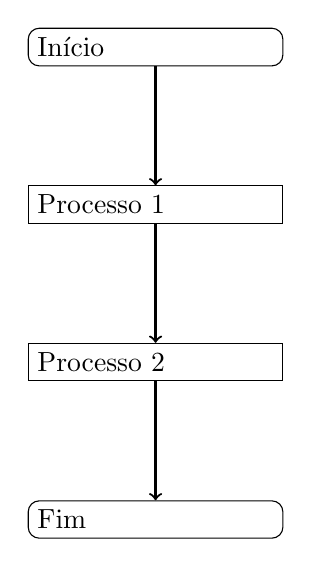
\begin{tikzpicture}[node distance=2cm]
\tikzstyle{startstop} = [rectangle, rounded corners, draw, text width=3cm]
\tikzstyle{process} = [rectangle, draw, text width=3cm]
\tikzstyle{arrow} = [thick,->]

\node (start) [startstop] {Início};
\node (pro1) [process, below of=start] {Processo 1};
\node (pro2) [process, below of=pro1] {Processo 2};
\node (end) [startstop, below of=pro2] {Fim};

\draw [arrow] (start) -- (pro1);
\draw [arrow] (pro1) -- (pro2);
\draw [arrow] (pro2) -- (end);
\end{tikzpicture}


\end{document}
